\chapter{Grundlagen und Technologien}
\label{cha:StandDerTechnik}

In diesem Kapitel werden die grundlegenden funktionalen Testmethoden beschrieben, welche in der Softwareentwicklung angewendet werden. Andere Testbereiche der Softwareentwicklung wie Performancetest und Penetrationstest werden hier nicht behandelt. Diese Arbeite zielt speziell auf die funktionalen Testmethoden ab und hat in diesem Bereich ihre Stärken, was aber nicht bedeutet, dass man dieselben Konzepte nicht auch für die anderen Testbereiche anwenden kann. \\
\\
Funktionale Tests haben die Aufgabe sicherzustellen, dass die Anforderungen aus der Spezifikation korrekt umgesetzt werden. Für die Umsetzung dieser Tests können sowohl manuelle als auch automatisierte Testmethoden verwendet werden. Die unterschiedlichen Methoden werden in diesem Kapitel genau beschrieben und auf die Unterschiede eingegangen.

\begin{figure}
\centering
\caption{Testmethoden unterteilt in White-Box und Black-Box-Testen}
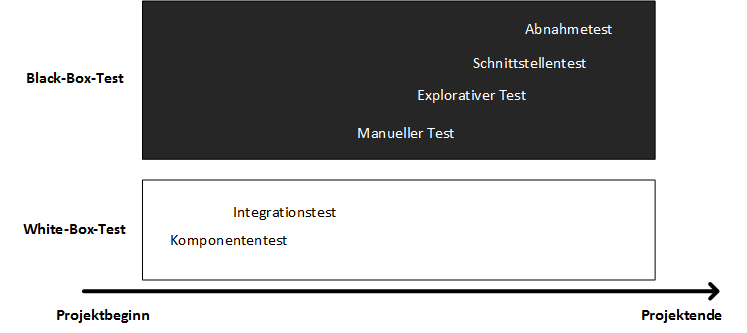
\includegraphics[width=0.9\textwidth]{testuebersicht.png}
\label{fig:testtypen}
\end{figure}

Im zweiten Teil dieses Kapitels werden die verwendeten Technologien beschrieben. Dazu gehören die Werkzeuge und Bibliotheken, welche für die Entwicklung der Sprache und der Ausführungseinheit verwendet werden. Weiters werden zwei Test-Treiber-Bibliotheken beschrieben, welche für automatisierte Abnahmetests verwendet werden können. 

\section{White-Box-Test}

Unter White-Box-Tests versteht man Tests, bei denen die Tester direkten Zugriff zu dem Quelltext haben. White-Box-Tests werden speziell für bestimmte Codefragmente geschrieben und testen typischerweise gezielt einzelne Fragmente einer Anwendung. Diese Tests werden in einer frühen Phase des Entwicklungsprozesses erstellt und liefern sehr bald eine messbare Qualitätskennzahl. \\
\\
Diese Tests sind typischerweise sehr technisch und verlangen vom Tester Programmierkenntnisse. Daher werden diese von den Entwicklern selbst geschrieben und fallen nicht in den Zuständigkeitsbereich des QA-Teams. Das gilt natürlich nur solange wir uns nicht in einem agilen Entwicklungsprozess befinden. Dort werden sowohl die White-Box- als auch die Black-Box-Tests im Entwicklungsteam umgesetzt.


\section{Black-Box-Test}

Die Gruppe der Black-Box-Tests sind klassisch in QA-Teams zu finden. Diese Gruppe umfasst alle Testansätze, bei denen der Quelltext der Anwendung nicht vorliegt. Für den Tester ist die Anwendung eine Blackbox. Die Aufgabe des Testers ist es zu überprüfen, ob alle Anforderungen laut Spezifikation umgesetzt worden sind. Für diese Aufgabe stehen dem Tester eine ganze Reihe an unterschiedlichen Ansätzen zur Auswahl, angefangen von manuellen Tests über explorative Tests zu automatisierten Abnahmetests. \\
\\
Die Black-Box-Tests werden typischerweise im fortgeschritten Projektstadium durchgeführt. Das ergibt sich aus der Tatsache, dass man für die Black-Box-Tests eine lauffähige Anwendung benötigt, welche durch den Tester benutzt werden kann.

\section{Manuelle Testmethoden}

Bei manuellen Tests handelt es sich generell um Black-Box-Tests. Dabei überprüft der Tester anhand der Spezifikation, ob sich die Anwendung korrekt verhält und ob die Funktionalität vollständig vorhanden ist. Die Funktionalität wird typischerweise über die Benutzeroberfläche geprüft. Eine zusätzliche Aufgabe bei manuellen Tests ist es, dass überprüft wird, ob die Benutzeroberflächen-Konzepte korrekt und einheitlich umgesetzt worden sind.\\
\\
Bei manuellen Tests ist es typisch, dass der Testmanager eine textuelle Beschreibung der Testfälle erstellt. Diese Testfälle werden dann von den Tester für jede neue Version der Anwendung durchgeführt. Bei einer Abweichung der Anwendung von den Testfällen muss der Tester entscheiden, ob sich der Anwendungsfall geändert hat oder ob die Anwendung nicht mehr korrekt funktioniert. Im letzteren Fall muss der Tester einen Fehlerbericht verfassen und an die Entwicklungsabteilung senden.

\subsection{Explorativer Test}

Eine Speziallform des manuellen Testens ist das explorative Testen. Dabei bekommt der Tester keine genaue Vorgabe, wie ein Testfall getestet werden soll. In diesem Fall bekommt der Tester eine Aufgabe, die er mit der Anwendung lösen muss. Das Ziel ist es, dass man unterschiedlichste Möglichkeiten der Anwendung testen kann. Dieser Ansatz ist gut dafür geeignet um neue Fehler zu finden. \\
\\
Grundsätzlich haben manuelle und auch automatisierte Tests die Limitierung, dass nur festgestellt werden kann, ob eine neue Version einer Anwendung gleich gut funktioniert wie die alte. Es können aber keine neuen Fehler abseits der definierten Tests gefunden werden. Diese Lücke versucht das explorative Testen zu schließen. Es ist auch von Vorteil, wenn nicht immer derselbe Tester dieselbe Aufgabe testet. Jeder Tester hat neue Ideen wie man die Aufgabe lösen kann und testet daher neue Bereiche und Kombinationen der Anwendung. Dieser Ansatz ist ein kreativer Prozess und kann daher im Gegenteil zu manuellen Tests nicht automatisiert werden.

\section{Automatisierte Testmethoden}

Das Ziel von automatisierten Tests ist es, dass man den Testaufwand in einem Software-Projekt reduziert. Aus wirtschaftlicher Sicht ist es viel besser, wenn das stupide Testen durch einen automatisierten Test erledigt wird. Bei manuellen Testern kann es bei mehrmaligen Wiederholungen eines Tests zu Aufmerksamkeitsverlusten kommen, was bei automatisierten Tests nicht der Fall ist.\\
\\
Durch automatisierte Tests werden Tester jedoch nicht obsolet. Auf der einen Seite müssen die automatisierten Tests auch von jemanden geschrieben und gewartet werden, auf der anderen Seite sind automatisierte Tests für exploratives Testen ungeeignet. Diese Aufgabe wird auf absehbare Zeit immer durch einen Tester erledigt werden.\\
\\
Schlussendlich gibt es noch einen weiteren wichtigen Vorteil von automatisierten Tests gegenüber manuellen Tests. Man kann automatisierte Tests viel öfters ausführen und sie liefern schneller eine Aussage über die Qualität der Software. Diese Zeitreduktion ist für agile Softwareprozesse sehr wichtig. Damit bekommen die Entwickler schneller eine Rückmeldung, ob das System noch korrekt funktioniert. 


\subsection{Komponententest (Unit Testing)}

Bei einem Komponententest wird genau eine Softwarekomponente getestet. Eine Softwarekomponente ist eine abgeschlossene Einheit in einem Software-Projekt, welche eine definierte Schnittstelle hat. Das kann zum Beispiel eine einzelne Klasse sein, aber auch ein ganzes Modul wie zum Beispiel in Pascal. Aus diesem Grund wird der Komponententest auch oft als Modul-Test oder Unit-Test bezeichnet. Dem Fall, dass die zu testende Komponente eine Abhängigkeit von einer anderen Komponenten hat, werden diese durch eine Test-Implementierung ersetzt. Der Vorteil von Komponententests ist, dass deren Erstellung und Wartung keinen großen Aufwand verursachen. Das ist auch der Grund, warum dieser Testansatz sehr beliebt und weit verbreitet ist. Die Beliebtheit dieser Variante kann man auch dadurch ablesen, dass es für so gut wie jede Programmiersprache ein Unit-Test-Bibliothek gibt. Der Vorteil ist aber auch zu gleich der größte Nachteil bei diesem Ansatz. Die Komponenten werden einzeln getestet und man kann daher keine Aussage darüber treffen, wie sich die das Gesamtsystem verhalten wird.\\
\\
Um eine Aussage über das Verhalten des Gesamtsystems zu bekommen, kann man im nächsten Schritt Integrationstests verwenden. Diese werden im nächsten Abschnitt erklärt.

\subsection{Integrationstest (Integration Testing)}

Der Integrationstest ist schon deutlich aufwendiger und umfangreicher als ein Komponententest. Bei einem Integrationstest werden alle Komponenten eines Softwaresystems gemeinsam getestet. Das Ziel bei diesen Tests ist es zu gewährleisten, dass alle Komponenten miteinander funktionieren und dass alle Schnittstellen korrekt implementiert worden sind. Es werden auch unterschiedliche Fehlersituationen im System simuliert und überprüft, ob diese ausgeglichen werden können. Ein einzelner Fehler in einer Komponente soll nicht das ganze System zum Absturz oder in einen ungültigen Zustand versetzen. \\
\\
Bei einem Integrationstest stellt sich oft die Frage, ob man mit oder ohne Datenbank testen soll. Diese Frage kann man nicht so einfach beantworten. Auf der einen Seite kann man sagen, dass die Datenbank genauso eine Komponente im Softwaresystem ist, welche getestet werden muss. Auf der anderen Seite kann man argumentieren, dass die Datenbank ein externes System ist, welches bereits getestet worden ist. Grundsätzlich ist jedoch zu sagen, dass es ein guter Ansatz ist, wenn man mit einer Datenbank die Integrationstests durchführt. Es kann immer wieder vorkommen, dass genau bei der Schnittstelle zwischen Softwaresystem und Datenbank Probleme auftreten. Diese Fehler würden sonst erst relativ spät im Projekt-Lebenszyklus auftreten und der Aufwand für die Behebung steigt.\\
\\
Der Grund warum über dieses Thema überhaupt so viel diskutiert wird ist, dass der Aufwand für einen Integrationstest mit Datenbank deutlich höher ist. Man muss sich eine Strategie überlegen, wie man für jede Testausführung einen definierten Datenbankzustand herstellen kann. Dieser Datenbankzustand ist sehr wichtig, um reproduzierbare Tests schreiben zu können. 


\subsection{Schnittstellentest (API Testing)}

Der Schnittstellentest ist die Vorstufe zum Abnahmetest. Dabei werden alle externen Schnittstellen getestet. Dabei kann es sich um eine Schnittstelle in ein externes System handeln oder auch um eine Webservice-Schnittstelle. Aber darunter fällt auch die Schnittstelle zwischen Benutzeroberfläche und dem Software-Backend. Diese Schnittstelle ist für Tester sehr interessant, da man hierbei die Benutzeroberfläche nicht für das Testen benötigt, jedoch das Gesamtsystem testen kann. Der Vorteil liegt darin, dass dieser Testansatz deutlich stabiler ist als ein Abnahmetest, welcher die Tests über die Benutzeroberfläche ausführt. Auch ist die Durchlaufzeit eines Schnittstellentests deutlich geringer als bei einem Abnahmetest.\\
\\
Der Unterschied zwischen einem Schnittstellentest und einem Integrationstest ist, dass bei einem Schnittstellentest das Software-System vollständig installiert wird. Für die Tests wird eine vollwertige Datenbank mit realistischen Demodaten verwendet. Bei einem Integrationstest verzichtet man auf diesen Aufwand.\\
\\
Wie schon die vorhergehenden Testansätze hat auch dieser Ansatz einen großen Nachteil. Bei diesen Tests werden nur die Schnittstellen zwischen externem System und der Benutzeroberfläche getestet. Dabei kann aber nicht sichergestellt werden, dass die Benutzeroberfläche fehlerfrei funktioniert. Für den Benutzer der Anwendung zählt schlussendlich nur, ob die Benutzeroberfläche korrekt funktioniert. Aus diesem Grund sind all diese Testansätze kein Ersatz für die Abnahmetests.

\subsection{Abnahmetest (User Acceptance Testing)}

Abnahmetests sind die aufwendigsten und kostenintensivsten Aufgaben im Testprozess. Bei einem Abnahmetest wird die Anwendung aus Sicht des Benutzers getestet. Der Tester verifiziert, ob alle Anwendungsfälle und Funktionen, welche in der Spezifikation definiert worden sind, vorhanden sind. Dafür muss eine lauffähige Anwendung vorhanden sein um diese Tests durchführen zu können. Im Wasserfall-Vorgehensmodell kommt dieser Testansatz am Ende des Entwicklungszyklus. Es kommt dabei nicht selten vor, dass der Kunde diese Tests manuell durchführt. Bei den agilen Vorgehensmodellen werden diese Tests nach jeder Iteration durchgeführt. Durch die kurzen Iterationszyklen können die Abnahmetests nicht mehr manuell durchgeführt werden. In diesem Fall kommen automatisierte Abnahmetests zum Einsatz. \\
\\
Die große Herausforderung bei diesem Testansatz ist es, die Balance zwischen manuellen und automatisierten Tests zu finden.

\section{Verwendete Technologien}

Rayden basiert auf und verwendet eine Vielzahl von unterschiedlichen Technologien, Werkzeugen und Bibliotheken. Dieser Abschnitt gibt einen Einblick in die Technologien und erklärt, in welchen Bereichen diese im Rayden-Framework verwendet werden. Als Basis wird die Programmiersprache Java und deren Laufzeitumgebung verwendet. Die Entscheidung für Java ist essentiell für das Projekt um eine große Anzahl an unterschiedlichen Test-Szenarien zu unterstützen. \\
\\
Für die Umsetzung der Sprache wurden viele Bibliotheken und Werkzeuge aus dem Eclipse-Umfeld verwendet. Als Test-Treiber-Bibliothek wird sowohl eine offene als auch eine kommerzielle Implementierung verwendet.\\

\subsection{Eclipse}

Eclipse ist eine Entwicklungsumgebung für eine Vielzahl an Programmiersprachen. Ursprünglich wurde Eclipse von der Firma IBM für die Sprache Java entwickelt. Im Laufe der Zeit wurde Eclipse zu einer beliebten Entwicklerplattform und es wurden immer mehr Sprachen über Plug-ins unterstützt. Auch für das Rayden-Framework soll ein solches Plug-in entwickelt werden um den Tester eine gute Unterstützung zum Erstellen von Tests bieten zu können. \\
\\
Neben der Entwicklungsumgebung ist Eclipse aber auch eine Plattform für die unterschiedlichsten Projekte geworden. Diese Projekte werden von der Eclipse Foundation verwaltet und durch Partnerunternehmen und freiwilligen Entwickler gepflegt. \\
\\
Einige dieser Projekte werden in den nächsten Abschnitten noch separat vorgestellt.

\subsection{EMF}

Das Eclipse Modeling Framework (EMF) ist ein Modellierungswerkzeug für Java. EMF stellte ein Set an Werkzeugen zur Erstellung, Verwaltung und Weiterverarbeitung zur Verfügung. Dazu gehört auch die Möglichkeit aus diesen Modellen Code zu generieren. Eine Kernkomponente von EMF ist das ECore-Metamodell. Ein Metamodell ist die Schablone für ein spezifisches Modell. Aus einem ECore-Modell kann man mithilfe von Code-Generatoren eine Java-Bibliothek generieren. \\
\\
Auf dieses Konzept baut auch das xText-Projekt auf, welches im nächstem Abschnitt vorgestellt wird. 

\subsection{xText}

Das xText-Projekt unterstützt das Erstellen von neuen Sprachen. Grundsätzlich ist xText ein Compiler-Generator der aus einer Grammatik einen lexikalischen und Syntax-Analysator generiert. Das besondere an xText ist aber, dass man noch zusätzlich eine Eclipse-Editor für die Sprache bekommt. Der Editor bietet grundlegende Funktionen wie Syntax-Highlighting, Fehler- und Validierungsmechanismen. Diese Funktionalität kann man nachträglich noch anpassen und weitere Funktionen hinzufügen. Ein Vorteil von xText ist, dass man den generierten Compiler nicht nur in Eclipse verwenden kann, sondern auch als eigenständige Anwendung ausführen kann. Somit erspart man sich den Aufwand zwei Compiler für seine Sprache zu warten. Der abstrakte Syntaxbaum einer Quelldatei wird im Compiler mit EMF umgesetzt. Das heißt man bekommt einen vollständigen Syntax-Baum im Hauptspeicher, welchen man sehr einfach verarbeiten kann. Um die Verwendung noch zu vereinfachen, liegt für den Baum ein Metamodell in Form eines ECore-Modells vor. 

\subsection{Selenium}

Selenium ist ein Open-Source Projekt um Webseiten automatisiert testen zu können. Die Bibliothek unterstützt eine Vielzahl an unterschiedlichen Browsern auf allen gängigen Betriebssystemen wie Windows, Linux, Mac und Google Android. Um die Browser ansprechen zu können benötigt man einen speziellen Treiber. Dieser wird entweder als separate Anwendung ausgeliefert oder bereits mit dem Browser mitgeliefert.\\
\\In der ersten Version hat Selenium auf einen propritären Programmierschnittstelle gesetzt. Seit der Version 2 setzt Selenium auf die standardisierte Programmierschnittstelle WebDriver vom W3C Konsortium. Der Vorteil von WebDriver ist, dass man eine einheitliche Programmierschnittstelle für die unterschiedlichsten Browser bekommt. Damit erzielt man eine rudimentäre Unabhängigkeit von einem spezifischen Browser. 

\subsection{Borland Silk Test}

Borland Silk Test ist eine kommerzielle Testsoftware für native wie auch Webanwendungen. Silk Test bietet eine Unterstützung für eine Vielzahl an unterschiedlichen Technologien. Unterstützt werden zum Beispiel die gängigen Browser wie Internet Explorer, Google Chrome und Mozilla Firefox. Neben Webtechnologien werden auch native Windows-Anwendung, Adobe Flex, WPF oder Java-Anwendungen unterstützt. Seit kurzem werden auch Mobile-Browser und -Anwendungen unterstützt. Der Vorteil von Silk Test gegenüber von Selenium ist, dass es einen X-Browser-Support gibt. Dabei kann man einen Test, welchen man mit dem Internet Explorer aufzeichnet, mit einem Mozilla Firefox oder dem Google Chrome Browser ausführen. Dasselbe funktioniert auch mit Desktop- und Mobile-Browser. Durch diese X-Browser-Technologie entfällt die Wartung von Tests für die verschiedensten Browser. 
